\chapter{Data, models and evaluation}
\label{chapter:Methods}


\section{Data}
\label{sec:data-and-features}


\subsection{The CHAMPS dataset}
\label{sec:champs-dataset}

This dataset has been published for the Kaggle competition 'Predicting Molecular Properties' organized by CHAMPS (CHemistry And Mathematics in Phase Space)~\footnote{\url{https://www.kaggle.com/c/champs-scalar-coupling/overview}}. The results from experiments using this dataset are presented in Section~\ref{sec:champs}.
	
The target variable is a magnetic interaction between two atoms measured by Nuclear Magnetic Resonance (NMR) - called scalar coupling constant or J-coupling constant~\cite{NMR}.
In graph notation, this represents an edge-property (see Section~\ref{sec:graph-output}). This interaction does not have to be predicted for any two atoms in the molecule, but rather for a predefined set of atom-pairs. These can be directly bonded to each other or be two or three covalent bonds apart. Furthermore, they can involve different atom types. The interactions are categorized into eight types by the involved atom types and the number of bonds between them. For instance, $2JHC$ is the J-coupling type of a hydrogen atom (H) and a carbon-atom (C) with two bonds between them.

The training-set contains 85012 molecular structures with 4659076 labeled J-coupling interactions, while the test has 45777 molecules with 2505190 relevant interactions (whose labels were not visible to the user at the time of the competition, but only used for automatic evaluation). The dataset was split on molecule level meaning that either all J-coupling interactions in a given molecule are part of the training set or all of them are in the test-set. For a more detailed investigation, please follow the links to two Kaggle-notebooks in the footnotes~\footnote{\url{https://www.kaggle.com/rpeer333/molecular-properties-detailed-eda}}
~\footnote{\url{https://www.kaggle.com/rpeer333/champs-competition-baseline-trivial-predictions}}.
In a general model, the J-coupling type would be the most important feature as the ranges of the J-coupling constant differ markedly between the eight types. However, a better approach is to train a different model for each type. This approach has been shown to be effective with boosted tree-models as well as MPNNs and was therefore used in both cases.

Apart from the raw structural data, the dataset also includes calculated chemical features. However, these are all just functions of the structural data and the J-coupling type and thus not used in the experiments at hand. The same approach was also chosen for the main dataset described in the next section.

The evaluation metric is based on the mean absolute error (MAE). As with the regular MAE, a lower score means better performance. The additional complexity serves the purpose of ensuring that all eight J-coupling types contribute roughly equally to the score.~\footnote{
	To understand this equation, note that the central element is $|y_i~-~\hat{y_i}|$ which is the absolute error for an individual J-coupling interaction, with $y_i$ being the real J-coupling constant and $\hat{y_i}$ the prediction. Keeping in mind that there are eight different kinds of J-coupling in the dataset, $n_t$ denotes the number of J-coupling interactions of type $t$. Thus, $~\frac{1}{n_t} \sum_{i=1}^{n_t}|y_i~-~\hat{y_i}|$ is simply the mean absolute error (MAE) of all J-coupling interactions of type $t$. Now, it is easy to see that the whole term is just the arithmetic mean of the log-MAEs of all eight J-coupling types. This somewhat more elaborate score is required because the number of interactions per J-coupling type varies considerably in the dataset. For the simple MAE over all J-coupling interactions, the score would be largely dominated by the more frequent J-coupling types, thus favoring a model focusing predominantly on those types. Calculating the log-MAE for all types independently and then averaging ensures a more equal contribution of all eight J-coupling types to the score. Finally, the only question remaining is, why the log-MAE is used instead of the simple MAE. The reason for this choice is most likely that the eight J-coupling types have very different variances. Thus, naturally, the MAE will be larger for the J-coupling types with larger variance. To avoid the score being dominated too much by those terms, the logarithm decreases the difference in contribution between low-variance and high-variance J-coupling types. Again, this leads to a more equal influence of the eight J-coupling types on the final score and requires the final model do reasonably well an all of them.
}\label{fn:score}

\begin{equation}\label{eq:champs-score}
	score = \frac{1}{8} ~ \sum_{t=1}^{8} ~ log(~\frac{1}{n_t} \sum_{i=1}^{n_t}|y_i~-~\hat{y_i}| ~)
\end{equation}



\subsection{The \textit{Alchemy} dataset}
\label{sec:alchemy-dataset}
The new quantum chemistry dataset \textit{Alchemy}, created by Tencent Quantum Lab~\cite{Chen2019}, was used for the bulk of the experiments in this thesis. The dataset is similar to the well established QM9 dataset~\cite{Ramakrishnan2014} with the same quantum mechanical properties as target variables and a similar number of molecules. The main advantage of the new \textit{Alchemy} dataset is that it also contains larger molecules of up to 12 heavy atoms (i.e., non-hydrogen atoms), as opposed to the maximum of seven heavy atoms in the QM9 dataset. This property makes it more relevant for medical research as potential drugs are not limited to only very small molecules. 
There are 119487 3D structures of molecules in the dataset. These structures provide the 3D coordinates as well as the atom-type (carbon, hydrogen, etc.) for each atom. Furthermore, the information which atoms are covalently bonded with each other and the type of the bond (single, double, triple) is also provided (even though this information could be calculated from the atom-coordinates if needed). Finally, twelve important quantum mechanical properties~\cite{Chen2019} are given for each molecule~\footnote{
	Unfortunately, due to the issue described in Section~\ref{sec:diff-old-new-ds}, the test set labels could not be used for reliable evaluation. The remaining dataset consists of 99776 molecules in the training-set and 3951 molecules in the validation set.
}. The task is to predict those twelve properties~\footnote{
	The 12 target variables
	(Dipole moment, Polarizability, HOMO, LUMO, gap, R\textsuperscript2, Zero point energy, Internal energy, Internal energy at 298.15 K, Enthalpy at 298.15 K, Free energy at 298.15 K, Heat capacity at 298.15 K) are shown in Table~2 of Chen et al.~\cite{Chen2019}.
} from the raw data.


%The target properties have been calculated using computationally highly expensive quantum chemical computations using the Python library \textit{PySCF}~\cite{Sun2017}.


\subsubsection{Features}
\label{sec:features}

There are two different approaches to predicting the target variables. The pure deep learning approach is to use only coordinates and bonds and rely on the model to learn any features required to predict the target properties. After all, coordinates, atom types and bonds contain all the available information (actually the bonds could be reliably calculated from coordinates and atom types and thus, strictly speaking are also redundant information).

The other approach is to calculate all sorts of chemical features using chemistry Python libraries and feed them into the model alongside the raw data. These include node (atom) features (whether the atom is an electron donor or acceptor, whether it is part of an aromatic ring, its hybridization type, etc.~\cite{Organic-chemistry}) as well as bond (edge) features. The fact that these features are calculated from the raw data without any additional information means that the model should also be able to learn them if required. Hence, calculating features and feeding them into the model should in theory be obsolete, but could slightly improve predictions if the model is unable to learn those features. Section~\ref{sec:raw-data} presents an experiment assessing the benefit of manually engineered features.

\subsubsection{Benchmark and evaluation}

The target variable in this dataset is a real-valued vector of length twelve. The error-metric used throughout this work is the mean absolute error (MAE) - which was also the metric in the competition. As the twelve quantum mechanical properties have vastly different ranges, they have to be normalized - otherwise the properties with larger ranges would contribute far more to the MAE than the properties with smaller ranges. Normalization was performed by subtracting the mean and dividing by the standard deviation.

\subsubsection{Difference between competition data and full data in the \textit{Alchemy} dataset}
\label{sec:diff-old-new-ds}

%This subsection explains why the MAE-values presented in this thesis cannot be compared the competition leader-board including my own score with rank 26.

\paragraph*{Overview} Unfortunately, the results obtained on the competition dataset cannot be directly compared to results achieved on the full dataset published after the \textit{Alchemy}-competition. This section presents the result of an investigation into the data quality issues and explains why the test-set (in particular the target variables) could not be used for the experiments. If the reader is only interested in the main topic of the thesis rather than inconsistencies in the particular dataset at hand, this subsection may be skipped. On the other hand, if the reader intends to train a model on this dataset, then reading this section can save a lot of time.

Figure~\ref{fig:competition-vs-full-ds} shows the learning curves of models being trained on both, the competition dataset and the full dataset. The MAE values are considerably lower on the competition dataset.

\paragraph*{Train-test split}
The competition dataset is split into training-set (called dev-set by the hosts), validation- and test-set with the ground truth being provided only for the first two sets. The split is not random. Instead, the validation- and test-set have an intentional bias towards larger molecules compared to the training-set. Building models that can extrapolate from smaller molecules to larger molecules is useful for pharmacological research~\cite{Chen2019}.
%However, in order to focus on the core topic of GCNN for molecules, for most experiments presented in this thesis. I only use a simple random split where training-, validation- and test-set are randomly drawn without replacement from the same population.

Figure~\ref{fig:competition-vs-full-ds} shows learning curves for both, competition-data split and random split to eliminate any differences in validation MAE hailing from the different dataset splits.
The figure shows two counter-intuitive results. First of all, the MAE is higher on the full dataset despite its larger size. Naturally, the larger dataset should give better or at least equally good results. Secondly, the impact of the splitting method varies between the two dataset. The expected result would have been a lower MAE on randomly split data because the training- and validation-molecules come from the same distribution. Having a strong bias towards higher weight molecules in the validation set is expected to increase the MAE. For the full dataset, this is indeed the case. However, for the competition dataset, the random split gives a higher MAE than the biased competition-split. As this result contradicts the expectation, it was thoroughly tested and validated.

%First of all, it is obvious that the validation MAE is lower on the randomly split data. This comes as no surprise because in the competition-data split, the validation molecules are systematically different (larger) from the training molecules. However, regardless of the kind of data-split, the MAE-values are still consistently lower on the competition data.


\begin{figure}[H]
	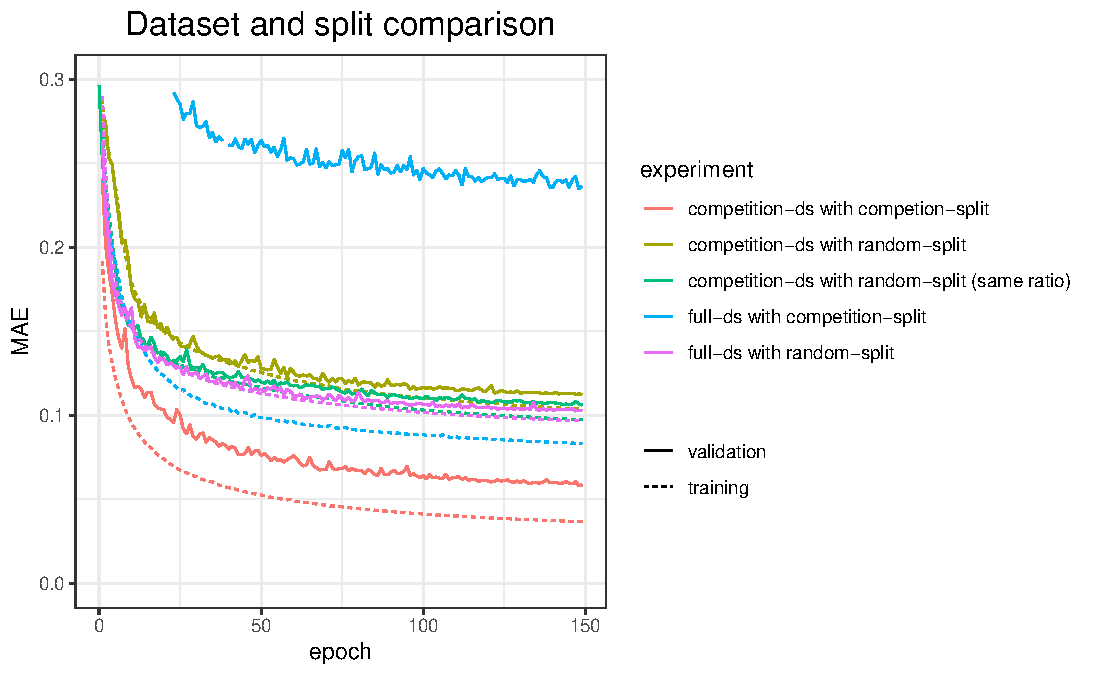
\includegraphics[width=\linewidth]{figures/competition-vs-full-ds}
	\caption{Comparing the full (post-competition) and the competition-dataset using various methods for splitting the data into training- and validation-set. Both datasets are evaluated using a random split (70\% training, 15\% validation, 15\% testing) and the train-validation split as it was defined in the competition (with a bias towards higher weight molecules in the validation set). In addition, the competition data is also subjected to a random split where the fraction of the validation-set is exactly the same as in the competition-data-split. (This last experiment was conducted to make sure that the observed difference is due to the method of splitting and not due to the size of the validation set.)}
	\label{fig:competition-vs-full-ds}
\end{figure}


\paragraph*{Target variable normalization}

In the competition dataset, the values are already normalized and the raw values are not available. It is not clear whether the mean and standard deviation used for normalization where calculated separately for the training- and validation-set or if the they are based on all molecules. Furthermore, the order of the target variables is unknown (by design) and their names are replaced with the dummy-names property-1, property-2, etc.

The full dataset released after the competition contains the raw values and the real names of the target variables. For training and evaluation, they were normalized in the same manner as in the competition (subtraction of mean and division by standard deviation). However, a direct comparison with the ranges of the competition dataset is not possible, as the names of the target variables are not provided there. 

%The only observation that can be made is that the average range (maximum - minimum) of all target variables is lower in the competition data-set. This suggest that the normalization might have been conducted on per-set basis because the range within a subset of the data is necessarily smaller or equal than the range of the full dataset. However, the small difference of an average range of 8.66 in the competition dataset and 9.72 in the full dataset is insufficient to explain the difference in MAE between the two datasets. Furthermore, such a difference could just as well be a function of dataset-size as larger datasets have a higher probability of containing more extreme outliers which increases the range of the target variables.

\paragraph*{Molecule data}

The raw data and thus the input into the model is exactly the same in the full dataset as in the competition dataset. This has been verified by thorough testing.

\paragraph*{Conclusion}

With the input-data as well as the data-splits being identical, the reason for the difference in MAE can only be explained by differences in the target variables. As discussed above, the absence of raw data in the competition dataset prevents a direct comparison of the target variables between the two datasets. Thus, no further information can be obtained to pinpoint the difference or to find a possible explanation. The only conclusion to be made is that for some reason the target variables in the new data prevent the model from learning to predict them as well as in the competition data. Therefore, only the training- and validation-set from the competition were used in the experiments. Furthermore, the same training-validation split as in the competition was chosen because the MAE of the competition-data with this split could not be achieved by any other splitting method. While it is unfortunate not to know the root of this counterintuitive finding, it will have to remain a mystery in order to focus on MPNNs, which are the core topic of this thesis.


\section{Model architecture}
\label{sec:architecture}

\subsection{\textit{SchNet}}
\label{sec:schnet-architecture}

As this model has not been used for many experiments, we shall refer to the literature for a detailed description. The implementation follows the architecture proposed by Schütt et al.~\cite{Schutt2017}. Several changes were made in this project's DGL-implementation~\footnote{\url{https://www.kaggle.com/rpeer333/pytorch-dgl-schnet-a-graph-convolutional-net}} compared to the template \textit{Chainer}-implementation~\footnote{\url{https://www.kaggle.com/toshik/schnet-starter-kit}}. In particular, a graph state was added. This is similar to the concept of a root- or master-node shown in Section~\ref{sec:root-node}. Furthermore, the residual short-cuts (first described in \textit{ResNets}~\cite{Sun2016}) in the graph convolution layers were replaced with dense short cuts analogous to the ones from \textit{DenseNets}~\cite{Huang2017}. Neither of those changes is responsible for the poor performance of the model, as the results were the same without them.


\subsection{Base MPNN architecture}
\label{sec:mpnn-architecture}

The basic architecture used as a starting point for most of the experiments in this thesis (Section~\ref{sec:alchemy}) comes from the MPNN variant from Chen et al.~\cite{Chen2019} whose code is available on GitHub~\footnote{\url{https://github.com/tencent-alchemy/Alchemy}}. This model, in turn, is based on the MPNN proposed by Gilmer et al.~\cite{Gilmer2017}.


\paragraph{Node embedding}The network starts with an embedding of the atom-type of each node. In this particular implementation, that is achieved by passing the one-hot encoded atom type through a regular linear layer. This first layer essentially extracts the n\textsuperscript{nt} column from the weight matrix when the n\textsuperscript{th} position of the input vector is one, which is easy to see from the following example.

\begin{equation}
\begin{bmatrix} 
w_{11} & w_{12} & w_{13} \\
w_{21} & w_{22} & w_{23} \\
w_{31} & w_{32} & w_{33} \\
\end{bmatrix}
*
\begin{bmatrix} 
1 \\
0 \\
0 \\
\end{bmatrix}
=
\begin{bmatrix} 
w_{11} \\
w_{21} \\
w_{31} \\
\end{bmatrix}
\end{equation}

Thus, the first linear layer essentially corresponds to a mapping from a categorical, integer-valued variable to a (learned) vector $\in \mathbb{R}^d$ where $d$ is the output dimension of the linear layer, which defines the dimension of the node hidden state.

\paragraph{Message passing}

The message passing function used in the experiments was the so called edge network message function, which was found to be the best among several options by Gilmer et al.~\cite{Gilmer2017}. The approach is described in detail and nicely illustrated by Simonovsky et al.~\cite{Simonovsky2017}. This message passing layer is implemented in the \textit{PyTorch Geometric} class NNConv~\footnote{\url{https://pytorch-geometric.readthedocs.io/en/latest/modules/nn.html\#torch_geometric.nn.conv.NNConv}}\label{fn:pytorch-geometric-nn-docs}.


The message function has two components. The first one is a two-layer MLP (multi-layer perceptron)  $h_{\mathbf{\Theta}}$ taking the edge features as input and outputting a vector of dimension $d^2$, which is reshaped into a $d$ by $d$ matrix (recall that $d$ is the dimension of the node hidden state).

\begin{equation}
	\Theta_{vw} = reshape(~h_{\Theta}(e_{vw})~)
\end{equation}

In the second step, the sending node representation $h_w$ is multiplied with this edge-conditioned weight matrix. Finally, an aggregation over all sending (neighboring) nodes gives the message for node $v$.

\begin{equation}
 m_v^{t+1} = \sum_{w \in \mathcal{N}(v)} h_w^t \cdot \Theta_{vw}
\end{equation}

It is easy to see how the two functions can be combined in a single message function. Finally, in the default setting, the update function is simply

\begin{equation}\label{eq:update-nnconv-simple}
	h_v^{t+1} = m_v^{t+1}
\end{equation}

If the root-node concept is used (by setting the parameter root-weight to 'True')\footnote{
	Technically, as Equation~\ref{eq:update-nnconv-root} shows, there is no root-node in this architecture. There is just the root weight-matrix $\Theta_{root}$, which can be thought of as a representation of an edge between the virtual root node and any real node in the graph. However, that is just an implementation-detail of this particular architecture. It is still valid to see $\Theta_{root}$ as the concept of a root node, which can be extended to other architectures as well.
}, the update function becomes

\begin{equation}\label{eq:update-nnconv-root}
h_v^{t+1} = \Theta_{root}h_v^t~+~m_v^{t+1}
\end{equation}



Oddly enough, in the simple case of Equation~\ref{eq:update-nnconv-simple}, the updated node hidden state $h_v^{t+1}$ is not a function of the previous hidden state $h_v^t$. While that is counter-intuitive, it was shown to work well in practice. Section~\ref{sec:root-node} compares the same model with and without the root-node and finds no difference in performance.

\paragraph{Readout function} Finally, the readout function is composed of a \textit{Set2Set}~\footnote{\url{https://pytorch-geometric.readthedocs.io/en/latest/modules/nn.html\#torch_geometric.nn.glob.Set2Set}} layer mapping the set of node hidden states to an aggregated representation. Then, the output from \textit{Set2Set} is mapped to the target variable with a two-layer MLP. The readout-function can be formalized as

\begin{equation}
		\hat{y} = MLP(~Set2Set(~\{~h_v^T\ ~|~ v \in G~\}~)~)
\end{equation}

\section{Software}

Most of the models presented in this thesis (Section~\ref{sec:alchemy}) were implemented using the Python deep learning library \textit{PyTorch}~\footnote{\url{https://pytorch.org/}} and its extension for graph neural networks, \textit{PyTorch Geometric}~\footnote{\url{https://pytorch-geometric.readthedocs.io/en/latest/}}. The \textit{SchNet} model (Section~\ref{sec:schnet}) was implemented using the Python library DGL (deep graph library)~\footnote{\url{https://www.dgl.ai/}}. In my humble opinion, \textit{PyTorch Geometric} is by far superior to DGL. Its API is much more in line with \textit{PyTorch}, the documentation is clear and the code works reliably. On the other hand, DGL is not straightforward to use and the work on the \textit{SchNet} model was severely hampered by a memory leak. In order to fix this issue, all caches had to be cleared after each batch leading to extremely slow training and making it impossible to try different approaches within limited time. Summing up, \textit{PyTorch Geometric} seems to be the best \textit{PyTorch}-compatible library for MPNNs.

The Python library \textit{mlflow}~\footnote{\url{https://mlflow.org/}} was used extensively to track all parameters and results for each experiment. It essentially creates a small local database containing all information the user wishes to save for each experiment. The data can be browsed via a dashboard or accessed via a Python API. This combination of automatic logging, a human readable dashboard and an API makes it the perfect tool for reproducible machine learning research and is highly recommended by the thesis author.

The code of the models trained on the \textit{Alchemy} dataset is available at github: \url{https://github.com/raph333/masters\_project}.



\section{Training}
\label{sec:training}

All experiments presented in this thesis use Adaptive Moment Estimation (Adam) for optimization~\cite{Kingma2015}. For certain experiments, other optimizers might give slightly better results. However, comparison between differences in data processing and model architectures would be impeded by employing different optimization schemes because one would never know if the different outcomes are a result of the model or the optimization. For this reason, optimization strategies were kept as constant as possible for all experiments.

The same considerations were applied to learning rates and learning rate scheduling. Two different optimization schemes were used for different purposes.
To obtain the lowest possible test-set error, a learning rate schedule that reduces the learning rate after the validation error plateaus has found to be most effective~\footnote{\label{fn:reduce-on-plateu}
	Specifically, the following parameters were chosen: The initial learning rate of 0.002 is reduced by a factor of 0.75 if the validation error did not decrease by a value of $10^{-4}$ or more within the last 8 epochs. The training duration was 300 epochs.
}. This optimization scheme suffers from the drawback of requiring many training epochs. Furthermore, the resulting learning-rate schedule varies considerably even between trainings with the same parameters (Figure~\ref{fig:optimization-variablility}a), which leads to considerable variation in the validation error (Figure~\ref{fig:optimization-variablility}b).

These differences as well as the long training time make it unsuitable for comparing learning curves with different parameters (however, it is a good strategy to achieve good results without spending a lot of time fine-tuning the optimization hyper-parameters).
For comparing different learning curves, a simpler, exponential learning rate decay was chosen~\footnote{
	The initial learning rate of 0.001 is reduced by a factor of 0.995 after every epoch and the experiment is run for 150 epochs.
}. The advantage of this method is that at each epoch, all curves have the same learning rate making them comparable. The final validation error is usually higher than would be achieved with reduce-on-plateau learning rate scheduling (furthermore, it also requires a few trials to find suitable hyper-parameters). However, this drawback is accepted because the main point of the experiments is to compare different model architectures, parameters or data-transformations rather than to achieve the lowest possible error.

%\begin{figure}[H]
%	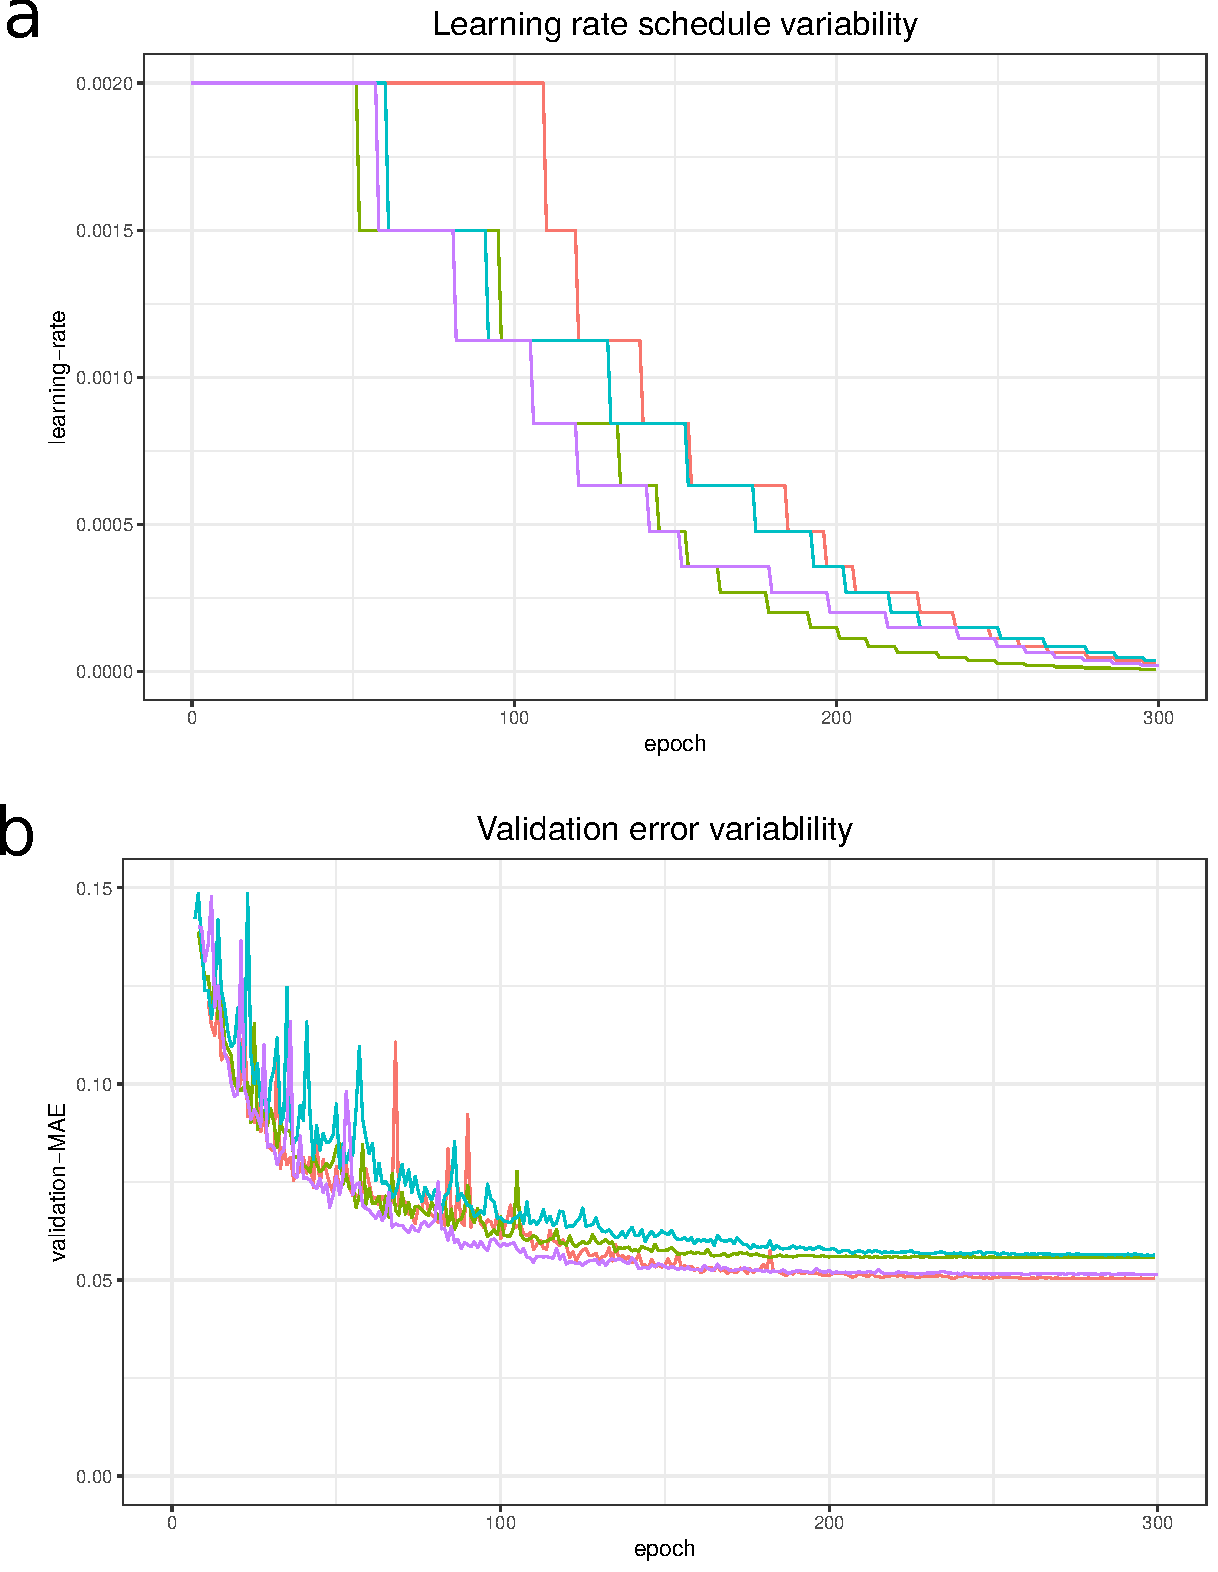
\includegraphics[width=0.9\linewidth]{figures/optimization-variabiliy}
%	\caption{The two graphs show metrics from four identical training runs with the reduce-on-plateau learning rate schedule using the parameters given in Footnote~\ref{fn:reduce-on-plateu}. Despite the same parameters, the resulting learning rate schedule varies markedly, as shown in \textbf{(a)}. The reason for this behavior is that small stochastic variations of the validation error early in the optimization determine when the learning rate is lowered first, which, in turn, influences the entire further optimization process. As a consequence, the resulting learning curves of the validation error also show substantial variation, as shown in \textbf{(b)}. Therefore, this optimization strategy is not well suited for comparing different models because it is not possible to determine whether the difference is due to the models or just the normal variation of this optimization schedule.}
%	\label{fig:optimization-variablility}
%\end{figure}


\begin{figure}[H]
	\begin{subfigure}{\textwidth}
		\centering
		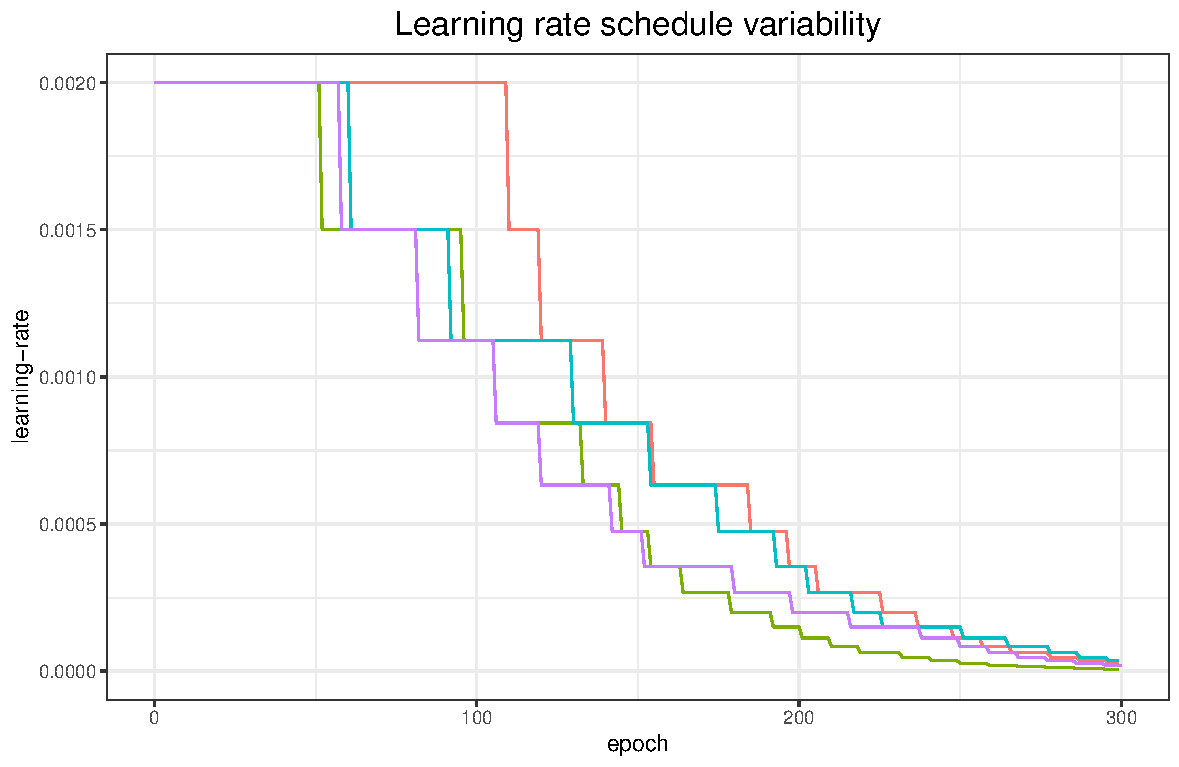
\includegraphics[width=0.9\textwidth]{figures/optimization-variablility-lr}
		\caption{}
		\label{fig:sub-a}
	\end{subfigure}
	\vfill
	\begin{subfigure}{\textwidth}
		\centering
		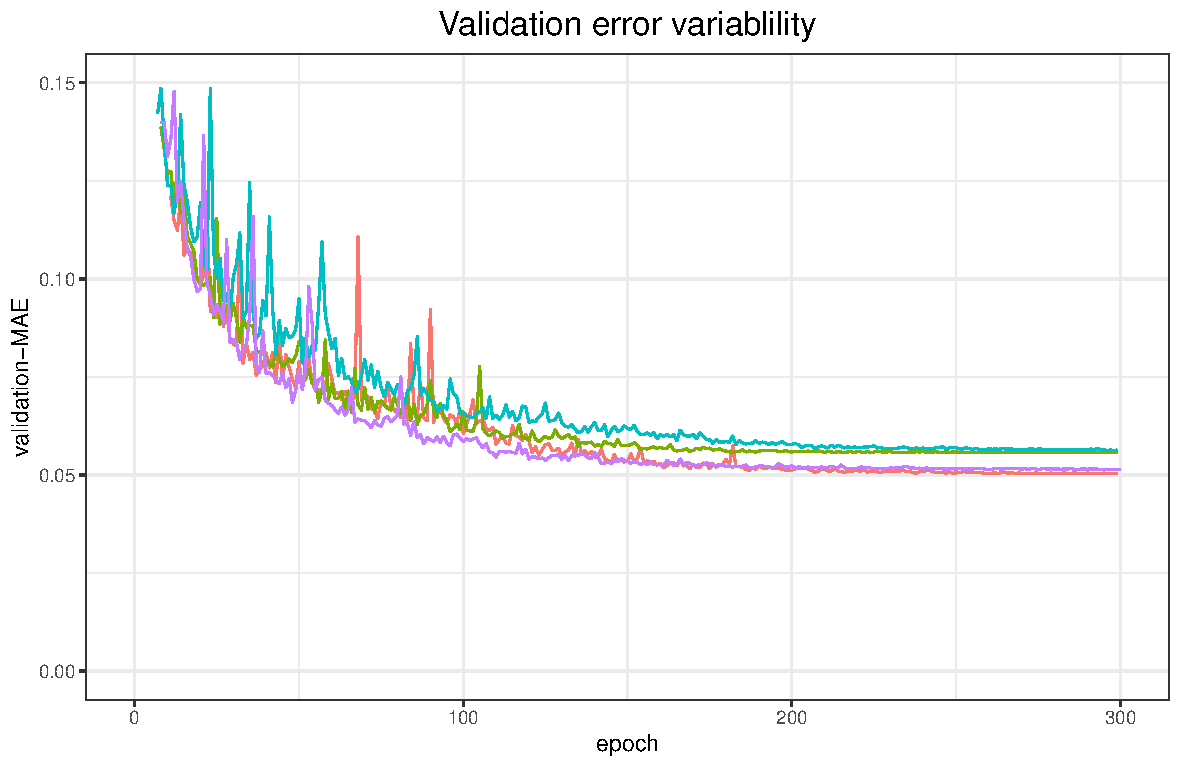
\includegraphics[width=0.9\textwidth]{figures/optimization-variablility-mae}
		\caption{}
		\label{fig:sub-b}
	\end{subfigure}
	\caption{The two graphs show metrics from four identical training runs with the reduce-on-plateau learning rate schedule using the parameters given in Footnote~\ref{fn:reduce-on-plateu}. Despite the same parameters, the resulting learning rate schedule varies markedly, as shown in \textbf{(a)}. The reason for this behavior is that small stochastic variations of the validation error early in the optimization determine when the learning rate is lowered first, which, in turn, influences the entire further optimization process. As a consequence, the resulting learning curves of the validation error also show substantial variation, as shown in \textbf{(b)}. Therefore, this optimization strategy is not well suited for comparing different models because it is not possible to determine whether the difference is due to the models or just the normal variation of this optimization schedule.}
	\label{fig:optimization-variablility}
\end{figure}

 
\section{Experiments}

Most experiments show learning curves with validation- and training-error rather than just the final errors. This choice was made because, in addition to showing the final error-rates, learning curves allow to estimate whether the model suffers from high bias (when the training-error plateaus and is not much better than the validation-	error) or high variance (when the training-error decreases rapidly, but the validation-error does not follow suit)~\cite{ml_yearning}. Furthermore, learning curves also indicate if prolonged training could lead to further improvements or if a plateau has been reached. In contrast, a single error-metric does not show how this metric was obtained and thus offers little information to interpret the results. Furthermore, learning curve averaging of multiple training runs was employed to reduce the impact of noise. Some variation in the learning curves is to be expected even in the absence of any difference in model architecture, input data or optimization strategy. Therefore, any learning curve shown in this thesis is an average of three independent learning curves using the exact same models parameters and input data. Conducting multiple training runs for each setting and averaging the results reduces the impact of random variation and allows to see the systematic differences instead. 

% appendix: interpreting learning curves

